\section{Technologies}

\subsection{Monitoring Techniques}

\subsubsection{Process Monitor}

One of the most basic forms of monitoring application is called system monitor \citep{WhatisaS27:online}, where the target application is monitored using the operating system's process manager which keeps track of resource usages from each of the running processes. This works well for small monolithic applications where typically there is only one application per server.

\subsubsection{Hypervisor Based Monitor}

Around the time of the early 2000s, a new way to manage servers called virtualization got popularized  \citep{Whatisvi12:online}. The idea behind this was to have one big server split into smaller isolated \ac{vm} which made sharing and managing hardware resources easier. To achieve this host computer runs software called Hypervisor which can create and delete guest \acp{vm} on demand \citep{Mergen_Uhlig_Krieger_Xenidis_2006}. As the hypervisor is responsible for managing the \ac{vm}'s resource requests, it can be used to observe the resource usage. Most cloud providers still rely on hypervisors to create \acp{vm} to sell to customers \citep{7waysweh13:online}. One of the most commonly used hypervisor is called Kernel-based Virtual Machine (KVM) which uses the Linux kernel itself as the  hypervisor, Which has a very small overhead on the host machine and grants better visibility into the guest system \citep{kivity2007kvm}.

\subsubsection{Service Mesh} \label{sec:service-mesh}

When the containerized distributed systems started getting popular both developers and operators were required to gather more insights about each application. Manually programming each application to collect telemetry is a time-consuming task and developers were reluctant to implement these. To overcome this challenge Service Meshes was introduced \citep{li2019service}. The idea behind this is to keep target service as it is and build a wrapper around it which will do all the instrumentation for the service. This is usually implemented as a side-car proxy \citep{Whatissi48:online}. 

\begin{figure}[H]
    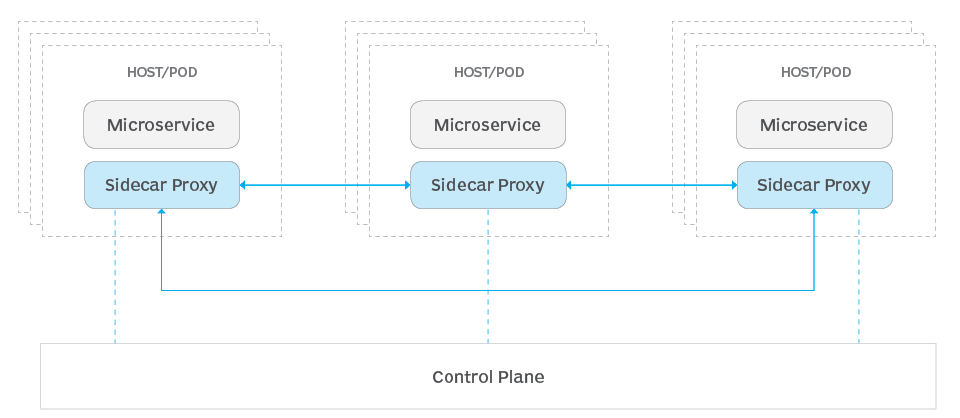
\includegraphics[width=16cm]{assets/literature-review/sidecar-proxy.png}
    \caption{Sidecar proxy design pattern \citep{Whatissi48:online}}
    \label{fig:sidecar-proxy}
    % https://cdn.ttgtmedia.com/rms/onlineimages/whatis-sidecar_proxy.png
\end{figure}

As this proxy sitting outside of the service, it is language-agnostic and intercepts all the inbound and outbound traffic at the application layer and relays them to responsible parties. This is a very effective method to provide a lot of visibility into services without requiring any additional work from the developers. The main problem with this approach is it adds a lot of both network and CPU overhead to analyze each of the requests with proxy \citep{Benchmar93:online}.

\begin{figure}[H]
    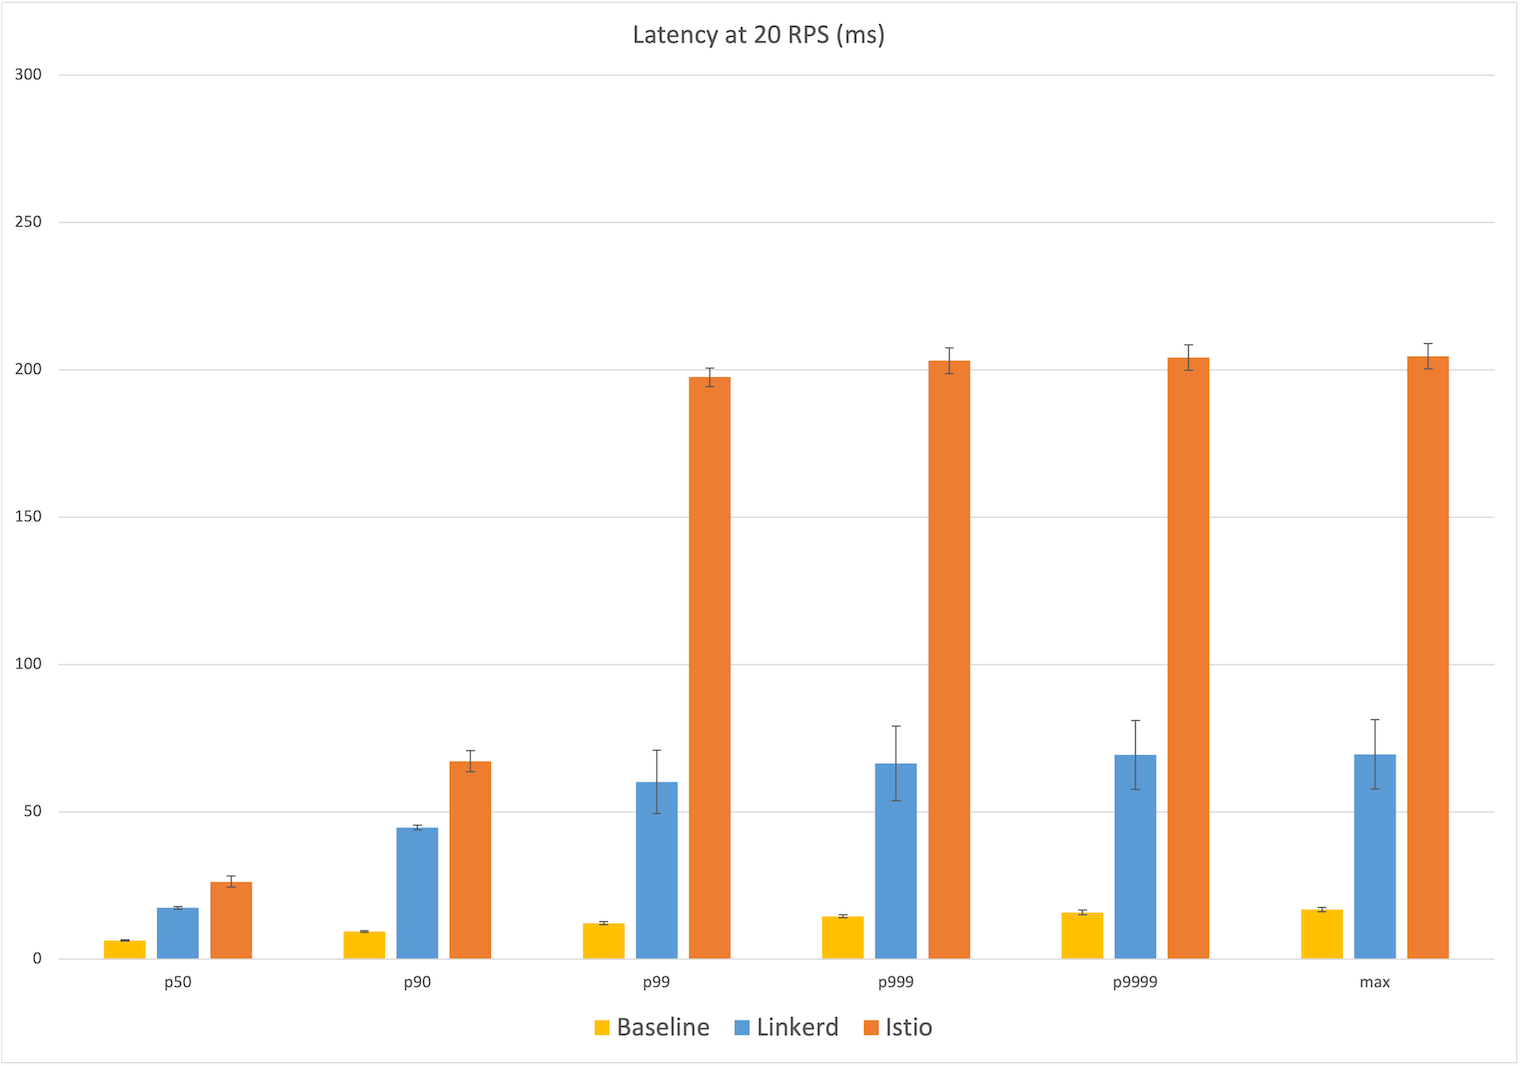
\includegraphics[width=11cm]{assets/literature-review/linkerd-benchmark.png}
    \caption{Service mesh benchmark \citep{Benchmar93:online}}
    \label{fig:linkerd-benchmark}
    % https://linkerd.io/images/benchmark/latency-20rps.png
\end{figure}

\subsubsection{Extended Berkeley Packet Filter (eBPF)}

\ac{ebpf} is a feature introduced to the Linux kernel in version 3.15 that allows deploying sandboxed programs to kernel space at run-time which could be used for application instrumentation from the kernel level \citep{LKMLIngo52:online}. \ac{ebpf} essentially created a way to run hooks on kernel events. For example kernel method "tcp\_v4\_syn\_recv\_sock" gets called every time a client wants to establish a TCP connection with the server. With \ac{ebpf} users can deploy a lightweight hook that is called every time a new connection is made which will update the state on \ac{ebpf} map which could be read from user-space. 

\begin{figure}[H]
    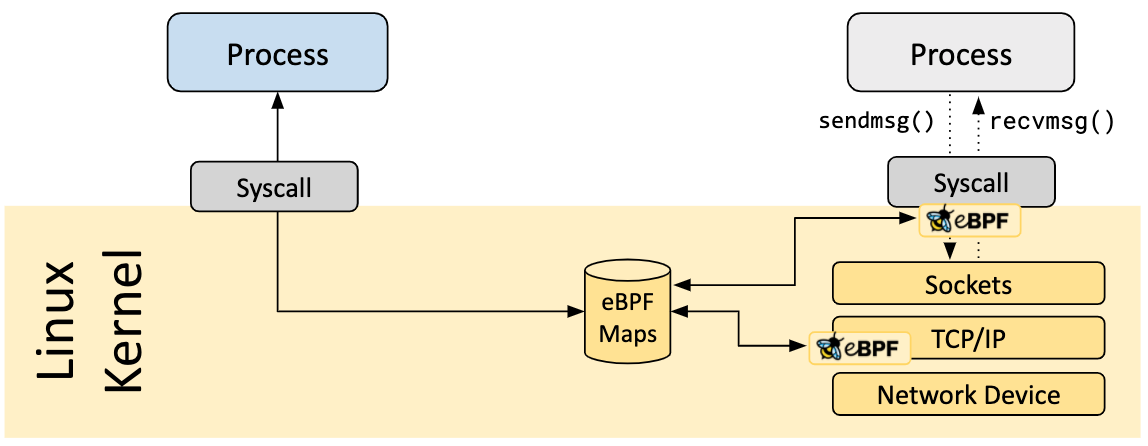
\includegraphics[width=11cm]{assets/literature-review/ebpf-architecture.png}
    \caption{eBPF architecture \citep{WhatiseB46:online}}
    \label{fig:ebpf-architecture}
    % https://ebpf.io/static/map\_architecture-e7909dc59d2b139b77f901fce04f60a1.png
\end{figure}

Using this data the request rate of a given service can be calculated with minimum overhead and zero instrumentation on the application. The main drawback of this method is it's very difficult to capture high-level data like HTTP status codes since those data only exist at the application level as it is.

\begin{longtable}{| p{23mm} | p{42mm} | p{42mm} | p{42mm} |}
\hline
    \textbf{Technique} &
    \textbf{Advantage} &
    \textbf{Disadvantage} &
    \textbf{Citations} \\ \hline

    Process Monitor &
    \vspace{-8mm}
    \begin{itemize}[leftmargin=0mm,noitemsep,nolistsep,label={}] 
        \item Virtually no overhead.
        \item Works out of the box.
        \vspace{-7mm}
    \end{itemize} &
    \vspace{-8mm}
    \begin{itemize}[leftmargin=0mm,noitemsep,nolistsep,label={}] 
        \item A very limited number of data points.
        \item     Not suited for a distributed system.
        \vspace{-7mm}
    \end{itemize} &
    \vspace{-8mm}
    \begin{itemize}[leftmargin=0mm,noitemsep,nolistsep,label={}] 
        \item \cite{chigurupati2017root}
        \item \cite{kumarage2018anomaly}
        \item \cite{kumarage2019generative}
        \vspace{-7mm}
    \end{itemize} \\ \hline

    Hypervisor Based Monitor &
    \vspace{-8mm}
    \begin{itemize}[leftmargin=0mm,noitemsep,nolistsep,label={}] 
        \item Most of the could providers gives simple API to access this data.
        \vspace{-7mm}
    \end{itemize} &
    \vspace{-8mm}
    \begin{itemize}[leftmargin=0mm,noitemsep,nolistsep,label={}] 
        \item A limited number of data points
        \vspace{-7mm}
    \end{itemize} &
    \vspace{-8mm}
    \begin{itemize}[leftmargin=0mm,noitemsep,nolistsep,label={}] 
        \item \cite{du2018anomaly}
        \item \cite{geethika2019anomaly}
        \vspace{-7mm}
    \end{itemize} \\ \hline
    
    Service Mesh &
    \vspace{-8mm}
    \begin{itemize}[leftmargin=0mm,noitemsep,nolistsep,label={}] 
        \item In-depth monitoring
        \item Request analyzing and modification at fly
        \item Framework Independent
        \vspace{-7mm}
    \end{itemize} &
    \vspace{-8mm}
    \begin{itemize}[leftmargin=0mm,noitemsep,nolistsep,label={}] 
        \item Performance Overhead
        \vspace{-7mm}
    \end{itemize} &
    \vspace{-8mm}
    \begin{itemize}[leftmargin=0mm,noitemsep,nolistsep,label={}] 
        \item \cite{samir2019dla}
        \item \cite{wu2020microrca}
        \vspace{-7mm}
    \end{itemize} \\ \hline
    
    Extended Berkeley Packet Filter &
    \vspace{-8mm}
    \begin{itemize}[leftmargin=0mm,noitemsep,nolistsep,label={}] 
        \item Very low overhead
        \item Works at the kernel level
        \item Able to scrape any data point related to the system
        \vspace{-7mm}
    \end{itemize} &
    \vspace{-8mm}
    \begin{itemize}[leftmargin=0mm,noitemsep,nolistsep,label={}] 
        \item Works only on Linux-based systems
        \item Difficult to develop and use
        \vspace{-7mm}
    \end{itemize} &
    \vspace{-8mm}
    \begin{itemize}[leftmargin=0mm,noitemsep,nolistsep,label={}] 
        \item None
        \vspace{-7mm}
    \end{itemize} \\ \hline

    \caption{Comparison of instrumentation methods (self-composed)}
\end{longtable}


\subsection{Detecting Anomalies}

\subsubsection{Supervised Learning}\label{sec:approch-supervised}
The most popular way to detect anomalies, in general, is using supervised learning methods. From finding outliers in sales patterns to fraud detection supervised learning methods can be implemented. \cite{du2018anomaly} mentioned even in the cloud computing domain still, more than half of the methods are relies on supervised learning to detect anomalies. Among these Support Vector Machines (SVMs), Random Forest and Decision Trees were used the most. But one of the main downsides to using supervised learning in cloud computing is the lack of labeled anomalous data. Since most of the systems nowadays target at least 99\% of uptime finding labeled data is difficult. Even if there is a well-balanced dataset, the trained model won't be able to recognize unforeseen anomalies.

\subsubsection{Semi-Supervised Learning}

As mentioned in \ref{sec:approch-supervised} one of the most challenging issues with anomaly detection is to find a dataset with enough labeled abnormal. One of the key contributing factors to developing a well-generalized model is having a well-balanced dataset \citep{batista2004study}. If the authors managed to find a sizable unbalanced dataset, using clustering algorithms like K-nearest Neighbors (KNN) could yield better results. \cite{akcay2018ganomaly} managed to utilized an encoder-decoder-encoder architectural model for detecting anomalies in image data and achieved remarkable results. 

\subsubsection{Unsupervised Learning}

When the target dataset consists of a lot of unlabeled data and it's difficult to label by hand, machine learning experts lean towards using unsupervised learning so the model can be its own teacher \citep{Unsuperv29:online}. \cite{silver2016mastering} managed to develop the first AI that was able to beat the best Go player in the world with a score of 4-1. This model learns to play the game of Go by look at thousands of games played by humans and learning to approximate the optimal strategy to any given board position. One year later same authors released the updated version of the model which learn to play Go without any human interference and this model beat the previously published model 100-0 \citep{silver2017mastering}. This proves deep learning models could even surpass humans when it comes to finding patterns in very large distributions. 

\begin{longtable}{| p{23mm} | p{42mm} | p{42mm} | p{42mm} |}
\hline
    \textbf{Technique} &
    \textbf{Advantage} &
    \textbf{Disadvantage} &
    \textbf{Citations} \\ \hline
    
    Supervised Learning &
    \vspace{-8mm}
    \begin{itemize}[leftmargin=0mm,noitemsep,nolistsep,label={}] 
        \item Easy to develop and train.
        \item Models will converge better to the dataset.
        \item Easy to test the model performance.
        \item Ideal used for classification and regression problems.
        \vspace{-7mm}
    \end{itemize} &
    \vspace{-8mm}
    \begin{itemize}[leftmargin=0mm,noitemsep,nolistsep,label={}] 
            \item Require a labeled dataset.
            \item The models won’t look at scenarios outside of the dataset. 
            \item The model will be biased if the labeled dataset was biased.
            \vspace{-7mm}
    \end{itemize} &
    \vspace{-8mm}
    \begin{itemize}[leftmargin=0mm,noitemsep,nolistsep,label={}] 
        \item \cite{du2018anomaly}
        \vspace{-7mm}
    \end{itemize} \\ \hline
    
    Semi-Supervised Learning &
    \vspace{-8mm}
    \begin{itemize}[leftmargin=0mm,noitemsep,nolistsep,label={}] 
        \item A blend of both Supervised and Unsupervised learning.
        \item Developers can force the model to learn some behaviors.
        \vspace{-7mm}
    \end{itemize} &
    \vspace{-8mm}
    \begin{itemize}[leftmargin=0mm,noitemsep,nolistsep,label={}] 
        \item Require a labeled dataset to train the initial steps.
        \item Model isn’t free to understand the problem from the ground up.
        \vspace{-7mm}
    \end{itemize} &
    \vspace{-8mm}
    \begin{itemize}[leftmargin=0mm,noitemsep,nolistsep,label={}] 
        \item \cite{akcay2018ganomaly}
        \vspace{-7mm}
    \end{itemize} \\ \hline
    
    Unsupervised Learning &
    \vspace{-8mm}
    \begin{itemize}[leftmargin=0mm,noitemsep,nolistsep,label={}] 
        \item Doesn’t require a labeled dataset.
        \item Excel at clustering extracting patterns from datasets.
        \vspace{-7mm}
    \end{itemize} &
    \vspace{-8mm}
    \begin{itemize}[leftmargin=0mm,noitemsep,nolistsep,label={}] 
        \item Developers have no control over the model’s behavior.
        \vspace{-7mm}
    \end{itemize} &
    \vspace{-8mm}
    \begin{itemize}[leftmargin=0mm,noitemsep,nolistsep,label={}] 
        \item \cite{kumarage2018anomaly}
        \item \cite{zhang2019deep}
        \item \cite{kumarage2019generative}
        \item \cite{khoshnevisan2019rsm}
        \vspace{-7mm}
    \end{itemize} \\ \hline
    \caption{Comparison of anomaly detect methods in distributed systems (self-composed)}
\end{longtable}

\subsection{Root Cause Identification}

It's very difficult to use a standard learning algorithms like Multilayer Perceptrons (MLP) to predict faulty service because the number of microservices in distributed systems changes frequently. Even if the system were to retrain the model after every new deployment it will hesitate to predict newly added services as the root cause since it doesn't have any historical data about the service to make assumptions. So almost all published research use either the Key Performance Indicator (KPI) correlation or some variations of graphs-based methods to predict the root cause of the failures \citep{soldani2021anomaly}.

\begin{longtable}{| p{23mm} | p{42mm} | p{42mm} | p{42mm} |}
\hline
    \textbf{Technique} &
    \textbf{Advantage} &
    \textbf{Disadvantage} &
    \textbf{Citations} \\ \hline
    
    KPI correlation &
    \vspace{-8mm}
    \begin{itemize}[leftmargin=0mm,noitemsep,nolistsep,label={}] 
        \item Could find indirectly affected services.
        \item Easy to implement.
        \vspace{-7mm}
    \end{itemize} &
    \vspace{-8mm}
    \begin{itemize}[leftmargin=0mm,noitemsep,nolistsep,label={}] 
            \item Search space is large.
            \item Could result in a lot of false positives and noisy outputs. 
            \vspace{-7mm}
    \end{itemize} &
    \vspace{-8mm}
    \begin{itemize}[leftmargin=0mm,noitemsep,nolistsep,label={}] 
        \item \cite{nguyen2011pal}
        \item \cite{nguyen2013fchain}
        \item \cite{wang2020root}
        \vspace{-7mm}
    \end{itemize} \\ \hline
    
    Graph-based methods &
    \vspace{-8mm}
    \begin{itemize}[leftmargin=0mm,noitemsep,nolistsep,label={}] 
        \item Gives clear visual reasoning for the predications.
        \item  
        \vspace{-7mm}
    \end{itemize} &
    \vspace{-8mm}
    \begin{itemize}[leftmargin=0mm,noitemsep,nolistsep,label={}] 
        \item Could miss out on indirectly affected components.
        \item Computing the causality graph could be expensive.
        \vspace{-7mm}
    \end{itemize} &
    \vspace{-8mm}
    \begin{itemize}[leftmargin=0mm,noitemsep,nolistsep,label={}] 
        \item \cite{samir2019dla}
        \item \cite{wu2020microrca}
        \item \cite{ma2020automap}
        \item \cite{meng2020localizing}
        \vspace{-7mm}
    \end{itemize} \\ \hline

    \caption{Comparison of root cause identification techniques (self-composed)}
\end{longtable}

\subsection{Evaluation}

Since this project consists of 3 components working together, all these can be evaluated separately and in the end as the whole system.

To evaluate an instrumentation system, the author is hoping to have use a static load generator like \href{https://github.com/MrSupiri/MicroSim}{MicroSim}. First a well established instrumentation system like linkerd will be installed and the static load generator will create some traffic. After the data is collected the proposed instrumentation system will be installed and same traffic  will be simulated. Finally the data from the first experiment will be collated with second to evaluate reliability of the instrumentation system.

Almost all the publication the author has reviews related to anomaly detection and root cause analysis, used three key evaluation metrics to measure the performance of these models, Precision, Recall, and F1 Score \citep{buckland1994relationship}. Precision denotes the proportion of correct positive classification (\( Precision = \frac{\text{True Positives}}{\text{True Positives} + \text{False Positives}} \)). In context of anomaly detection, how many events were actually anomalous over the models anomalous predictions. After training if the model had 1.0 as the precision which means model generated zero false positives. Recall in the other hand the exact opposite of this, It tries to identify from all the predictions how many were false negative (\( Recall = \frac{\text{True Positives}}{\text{True Positives} + \text{False Negatives}} \)). Problem with these two metrics are both it only explain the part of the story. For example model can have 1.0 precision by classifying all the things as non anomalous, If the test dataset is biased towards non anomalous then precision will get an artificial boost since model is rewarded more for getting false negatives. In order to fix that problem F1 score can be used. F1 score seeks a balance between both precision and recall and F1 score (\( F1 = 2*\frac{Precision*Recall}{Precision+Recall} \)) generally gives a better insights about classification models when there is imbalanced class distribution in the dataset \citep{Accuracy18:online}.
